\documentclass{article}

\usepackage[a4paper, total={6in, 8in}]{geometry}

\usepackage{amsmath}
\usepackage{amsfonts}
\usepackage{amssymb}
\usepackage[T1, T2A]{fontenc}
\usepackage[utf8]{inputenc}
\usepackage[english, russian]{babel}
\usepackage{graphics}
\usepackage{graphicx}

\geometry{
 a4paper,
 total={170mm,257mm},
 left=20mm,
 top=20mm,
 }

\author{Александр Валентинов}
\title{Лабораторная работа 3.6.1}

\begin{document}
   \subsection*{Работа 3.3.4}
   \section*{Эффект Холла в полупроводниках}
   
   \paragraph{Цель работы:} измерение подвижности и концентрации носителей заряда в полупроводниках.
   
   \paragraph{В работе используются:} электромагнит с источником питания, амперметр, миллиамперметр, милливеберметр, реостат, цифровой вольтметр, источник питания ($1.5$В), образцы легированного германия.
   
   \subsubsection*{Экспериментальная установка:}
   
   \begin{figure}[h]
   \centering
   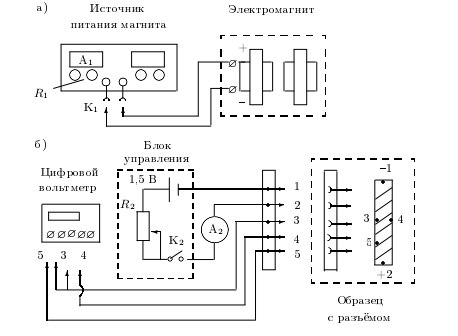
\includegraphics[width=8cm]{3_3_4.jpg} 
   \caption{Схема установки для исследования эффекта Холла в полупроводниках} 
   \label{fig.1} 
   \end{figure}

   \vfill
   \pagebreak


\end{document}
